\section{Hinführung}

In diesem Abschnitt werden die Lesenden in das Thema nutzungsorientierte Gestaltung eingeführt.
Hierzu wird der Begriff definiert, wichtige Aspekte der nutzungsorientierten Gestaltung herausgestellt und ihr Ablauf beschrieben.
Schlussendlich wird auf die Wichtigkeit der nutzungsorientierten Gestaltung für die Informatik eingegangen.

\subsection{Definition}\label{sec:definition}

Das traditionelle Vorgehen in der Softwareentwicklung ist es, von der Technik hin zum Menschen zu denken.
Dies ist für viele Entwickelnde einfach, da das entstehende Produkt so im Laufe des Entwicklungsprozesses an die verfügbare Technik angepasst werden kann.
Nutzungsorientierte Gestaltung (NOG) bricht mit dieser Vorgehensweise.

\begin{quote}
User-Centered Design (hier: Nutzungsorientierte Gestaltung, Anm.d.Auth) ist ein Konzept der Produktentwicklung und -gestaltung, das die Nutzerbedürfnisse in den Mittelpunkt des Entwicklungsprozesses rückt, um ein eine optimale User Experience zu ermöglichen. \cite{IONOS_nog_def}
\end{quote}

Zu erkennen ist, dass NOG die Nutzenden der Software schon bei der Entwicklung in den Mittelpunkt stellt.
Hierfür muss ein entwickeltes System Funktionen bereitstellen, welche den Arbeitsalltag erleichtern und nicht nur ihre technischen Anforderungen erfüllen.
Es soll also "verständlich, handhabbar, erlernbar [und] intuitiv" \cite{NOG} sein. 
Dies kann durch Usability Engineering, sowie dem Fokus auf Benutzerschnittstellen und der Mensch-Maschine Interaktion erreicht werden.
Hierbei gilt es einige Kriterien einzuhalten:

\textbf{Aufgabenangemessenheit} sieht vor, dass die entstehende Software genau dem Problem angemessen ist.
Dabei soll sie alle benötigten Funktionen enthalten, darüber hinaus aber keine weitere, für die Nutzenden störende oder verwirrende, Funktionen besitzen.
Es weiteren wird versucht die Anzahl an Mensch-Maschine Interaktionen auf ein Mindestmaß zu reduzieren.

\textbf{Selbstbeschreibungsfähigkeit} verlangt vom System, dass Nutzende das System ohne längere Einführung durch Dritte sofort nutzen und verstehen können.
Dazu können System eigene Hilfen und Rückmeldungen implementiert werden.

\textbf{Lernförderlichkeit} liegt in direktem Zusammenhang zur Selbstbeschreibungsfähigkeit.
Bei größeren Systemen für komplexere Anwendungsfälle ist eine vollständige Selbsterklärung der Systeme nur schwer möglich.
Trotzdem sollen Systeme den Lernprozess unterstützen.
Beispielsweise kann eine Software, wie bei Videospielen üblich, über ein Tutorial zum Erlernen dieser verfügen.

\textbf{Steuerbarkeit} bedeutet, dass die Mensch-Maschine Interaktion durch die Nutzenden initiiert werden soll.
Diese müssen zu jedem Zeitpunkt das System steuern.
Dieses darf keine unerwarteten, eigenen Aktionen durchführen.

\textbf{Erwartungskonformität} bezieht sich auf das verhalten den Systems.
Dieses soll an das erwartete Verhalten der Nutzenden angepasst werden, wobei auch stark der Nutzungskontext beachtet werden muss.
Ebenso ist eine konsistente Gestaltung der Funktionen wichtig.

\textbf{Fehlertoleranz} erlaubt es den Nutzenden trotz nicht vermeidbarer Eingabefehler weiterhin eine gute bis optimale Experience zu erlangen.
Dafür muss das System die Nutzenden entweder auf Fehler aufmerksam machen oder, sollten diese unentdeckt bleiben, ohne fatale Fehler mit den Eingaben arbeiten können.

\textbf{Individualisierbarkeit} ermöglicht es den Nutzenden das System genau für ihren konkreten Arbeitskontext anzupassen. 
Da sich dieser von Situation zu Situation andern kann, soll diese Individualisierbarkeit leicht zugänglich und umzusetzen sein.

NOG ist also mehr als nur Oberflächengestaltung.
Deshalb beinhaltet der nutzungsorientierte Prozess multi-disziplinären Aspekte von Design, Softwareentwicklung und Sozialwissenschaften.

Diesen Aufwand belohnt NOG durch eine Qualitätsverbesserung, Akzeptanzerhöhung und gleichzeitig eine, durch die Einbindung der Nutzenden resultierende, Vermeidung technischer Fehlentwicklungen.

\subsection{Prozessablauf}\label{sec:prozessablauf}

NOG ist als Kreislauf aus Verstehen, Definieren, Gestalten und Evaluieren zu verstehen.
Dieser Kreislauf wird viele Male durchlaufen, bis am Ende ein den nutzungsorientieren Anforderungen entsprechendes Resultat entsteht.

Der Ablauf des nutzungsorientierten Prozesses ist in \autoref{fig:nog_process} als linearer Prozess zu sehen.
Im Folgenden wird dieser genauer beleuchtet und aufgezeigt, an welchen Stellen sich dort der soeben benannte Kreislauf auffinden lässt.
Die im Zuge dieser Auflistung erwähnten Methoden werden unter \autoref{sec:methoden} genauer erklärt.

\begin{figure}[htp]
    \centering
    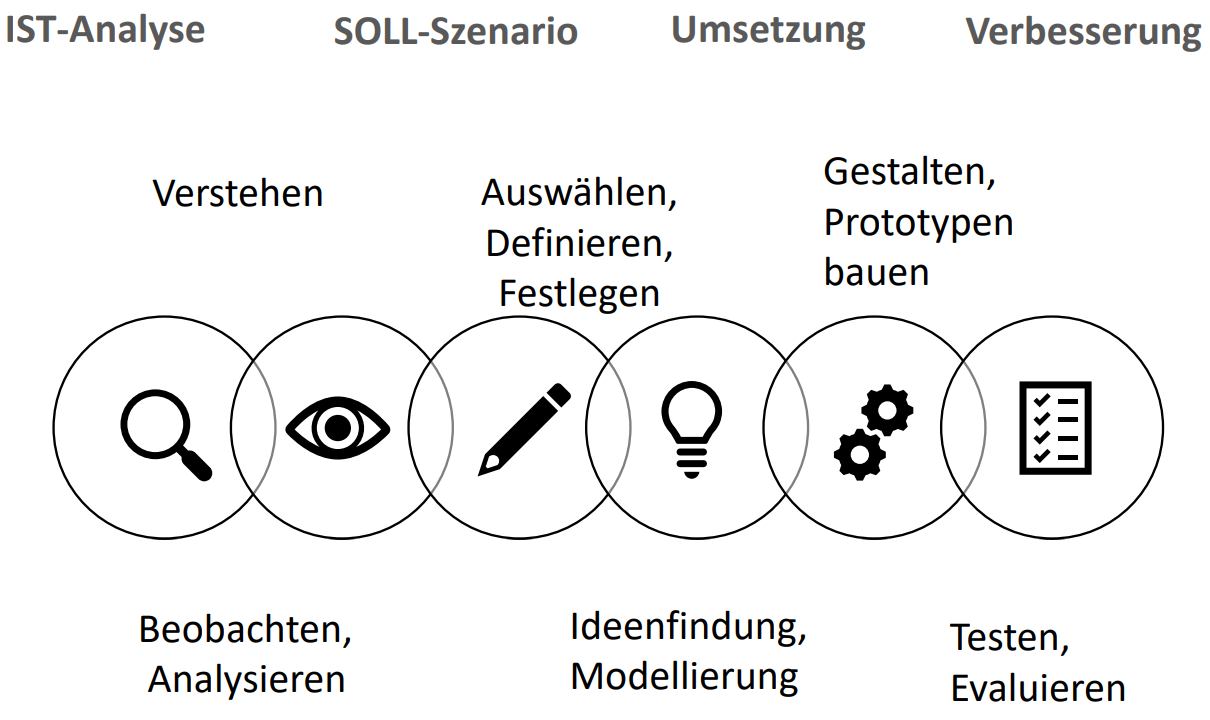
\includegraphics[width=1\textwidth]{images/NOG_Prozess.png}
    \caption{Ablauf des nutzungsorientierten Prozesses}
    \label{fig:nog_process}
\end{figure}

\autoref{fig:nog_process} verwendet für den oben benannten Kreislauf die Begriffe IST-Analyse, SOLL-Szenario, Umsetzung und Verbesserung. 
Diese Vorgänge seien nun aufgelistet und beschrieben.

\subsubsection{IST-Analyse}

In diesem ersten Abschnitt der NOG geht es darum, den vorherrschenden Kontext zu verstehen.
Dies ist essenziell um nutzerzentrierte Software zu entwickeln.
Um die Tätigkeiten und Abläufe des Kontextes zu verstehen, wird zunächst Kontakt zu Personen aus dem konkreten Nutzungskontext aufgenommen.
Mit einer oder mehreren dieser Personen wird ein Interview im Kontext durchgeführt.
Eine Erläuterung dieser Methode ist \autoref{sec:interview} zu entnehmen.
Ebenso werden zu diesen Zeitpunkt Contextual Design Modelle herangezogen, damit weiter in den Kontext eingestiegen werden kann und dieser besser verstanden wird.
Eine Erläuterung zu Contextual Design Modellen ist in \autoref{sec:modelle} zu finden.

Auf Basis der erlernten Informationen über den Kontext werden sodann sogenannte Personas, fiktive, den typischen zukünftigen Nutzenden der Software entsprechenden, Personen erstellt.
Eine Erläuterung des Konzepts der Persona findet sich in \autoref{sec:persona}.
Schlussendlich werden ein oder mehrerer IST-Szenarien verfasst, welche die vorherrschenden Abläufe des Kontextes, durchgeführt durch die zuvor erstellten Personas, zusammenfasst.
Auch eine Erläuterung zu Szenarios ist im Folgenden zu finden.
Sie ist \autoref{sec:sezenarien} zu entnehmen.

\subsubsection{SOLL-Szenario}

Im zweiten Schritt der NOG soll auf Basis der IST-Analyse ein SOLL-Szenario erarbeitet werden. 
Dieses SOLL-Szenario, beziehungsweise diese SOLL-Szenarien, basieren auf den IST-Szenarien.
Nun verfügen die Handelnden jedoch über die zu entwickelnde Software als Hilfestellung für ihre Tätigkeit.
Bei der Erstellung dieser Szenarien ist darauf zu achten, dass die Aspekte der NOG eingehalten werden.
Sie bilden das Fundament für die weitere Entwicklung der Software.

\subsubsection{Umsetzung}

Dieser dritte Schritt im Prozess der NOG nutzt die gesammelten Informationen und Ideen der IST- und SOLL-Analysen um darauf aufbauend einen Prototyp für das fertige Produkt zu erstellen.
Diese Prototypen können in verschiedenen Formen erstellt werden.
Weitere Infos hierzu ist \autoref{sec:prototypen} zu entnehmen.
Auch hierbei ist, sogar noch intensiver als im Zuge der SOLL-Szenarien, darauf zu achten, dass alle Prinzipien und Aspekte der NOG eingehalten werden.

\subsubsection{Verbesserung}

In diesem Schritt wird die bisher geleistete Arbeit den Kontextpersonen vorgestellt.
Damit diese einen möglichst guten Einblick in die Ideen und Lösungen der Entwickelnden haben, müssen letztere so realistische Prototypen wie möglich erarbeiten.
Nach einer Vorstellung der Prototypen können die Kontextpersonen Rückmeldungen über das erarbeitete Konzept geben.
Je nach Art des Prototypen kann dieser auch praktisch im Kontext erprobt werden.

Mit der Rückmeldung der Kontextpersonen schließt sich der am Anfang des Kapitels angesprochene Kreis der NOG.
Die Entwickelnden begeben sich mit dem aus den Rückmeldungen gewonnen Wissen zurück zum Schritt des SOLL-Szenarios oder der Umsetzung, damit die gewünschten Änderungen dort eingearbeitet werden können.
Diese iterative Entwicklung des Produkts hält an, bis dieses dem Anspruch und Nutzen der Nutzenden gewachsen ist.

\newpage
\subsection{Wichtigkeit}

Zum Schluss dieses Abschnittes sei noch einmal die Wichtigkeit von nutzungsorientierter Gestaltung für die Informatik betont.
Bereits zu Beginn wurde erwähnt, dass der traditionelle Ansatz der Softwareentwicklung von der Maschine hin zum Menschen arbeitet.
Da die Software jedoch am schlussendlich von Menschen verwendet werden soll, hat dieser Ansatz nicht den besten praktischen Nutzen.
Ein auf diese zugeschnittenes digitales System kann nicht nur das Wohlbefinden, sondern auch die Produktivität der Nutzenden steigern \cite{NOG}.
Ein weiterer Vorteil der Einbindung von Nutzenden in die Entwicklung der Software ist, dass diese dem Resultat offener gegenüber stehen.
Oft haben Personen, welche längere Zeit eine Tätigkeit auf die selbe Weise ausführen keine Toleranz für (technische) Änderungen an ihren Arbeitsabläufen.
Arbeiten diese Personen jedoch direkt an der zu verwendenden Technik mit, so so reduziert sich diese Barriere auf ein Minimum.